\documentclass[12pt]{article}
\usepackage[margin=1in]{geometry}
\usepackage{graphicx}
\usepackage{amsmath,amssymb}
\pagestyle{empty}
\begin{document}

\begin{center}
\textbf{\large Online Resource 3}
\end{center}
\vspace{0.5em}

\begin{center}
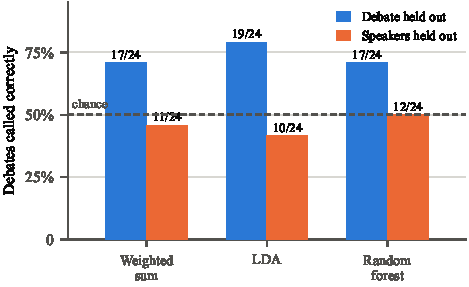
\includegraphics[width=0.85\textwidth]{fig_holdout.pdf}
\end{center}

\vspace{1em}
\noindent\textbf{Caption.} Debate-level accuracy of three classical models
(weighted sum, linear discriminant, decision forest) reported in Table~9 of
the main text, evaluated two ways. Holding out the debate leaves both of its
speakers in the training data; holding out the speakers removes them
entirely. All three models fall to chance under the stricter test. This
figure presents, in visual form, the same comparison tabulated in Table~9 of
the main text.

\end{document}
